% Setup - do not change
\documentclass[11pt]{article}
\usepackage[top=0.9in, left=0.9in, bottom=0.9in, right=0.9in]{geometry} 
\usepackage{parskip}
\usepackage{subfigure}
\usepackage[english]{babel}
\usepackage[utf8]{inputenc}
\usepackage{amsmath,amsthm,amssymb,graphicx,pdfpages,lipsum,hyperref}
\usepackage[none]{hyphenat}
\usepackage{csquotes}

\setlength\parindent{0pt}
%%%%%%%%%%%%%%%%%%%%%%%%%%%%%%%%%%%%%%%%%%%%%%%%%%%%%%%%%%%%%%%%%%%
% add other packages here if required

%% Bibliography are specified in this file. You can also choose inline bib style if you want to. But make sure your citation style is consistent (and proper)
% For more details on citation: https://library.unimelb.edu.au/recite
\usepackage[sorting = none]{biblatex}
\addbibresource{references.bib}

%%%%%%%%%%%%%%%%%%%%%%%%%%%%%%%%%%%%%%%%%%%%%%%%%%%%%%%%%%%%%%%%%%% the '%' symbol denotes comments

% Begin document creation
% DELETE THE \lipsum PLACEHOLDERS WHEN YOU BEGIN
\title{\textbf{Analysing of Taxi Demand over Spatial and Temporal in NYC}}
\author{
Insert Student Name:Mingrui Chen\\
Student ID: 1135354 \\
\href{https://github.com/MAST30034-Applied-Data-Science/mast30034-project-1-Albert-CHEN612.git}{Github repo with commit}
}

\begin{document}
\maketitle

\section{Introduction}
Taxi demand analysis is an important application of transportation systems in smart city construction, which provides crucial information in decision-making for transportation departments to upgrade their road network and taxi companies to make an effective strategy \cite{yao2018deep}.
Existing work predicts taxi demand using real-time population generated by cellular networks \cite{ishiguro2018taxi}, however, population density cannot be directly considered as taxi demand due to differences in multiple scenarios such as daytime and nighttime. 

Figure \ref{Fig:demand_num} shows the average frequency of yellow and green taxi trips on one day during January 2016. As shown in Figure \ref{Fig:demand_num}, both yellow taxis and green taxis show different quantities of trips in the daytime and nighttime. There is an increase in taxi demand from 6am to 9am. After the morning peak, the taxi demand is stable during the daytime until the evening peak comes from 5pm to 7pm. After that, the taxi demand decreases along with the time until 6 a.m. the next day.


\begin{figure}[b]
\includegraphics[width=0.7\textwidth]{plots/average_trips_time.pdf}
\centering
\caption{Yellow taxi demand in March 1 2016}
\label{Fig:demand_num}
\end{figure}


Figure \ref{Fig:demand_loc_5pm} and Figure \ref{Fig:demand_loc_6am} shows the average demand of taxi service in different area in NYC at 5pm and 6am in January 2016 over yellow taxi, respectively. As we can see in Figure \ref{Fig:demand_loc_6am} the demand for taxis at midnight in different locations shows a clear difference from that at 6am. We can learn that for taxi demand in workdays, 6 am is the beginning of the morning peak and taxi demand will increase from 6 am. 5pm is at the beginning of the evening peak in the daytime. The location with the most taxi demand in the morning is different from that in the evening. In addition, green taxis show different distribution than yellow taxis. In the suburbs, yellow taxi demand is higher than green taxi demand, whereas yellow taxi demand is higher in the CBD. This observation helps us learn the direction of the most busy trips between locations and gives us the idea of constructing a better transportation network. Thus, both spatial and temporal are needed to consider in predicting taxi demand in NYC.


\begin{figure}[t]
\centering
\begin{minipage}{0.85\linewidth}
\begin{subfigure}{\linewidth}
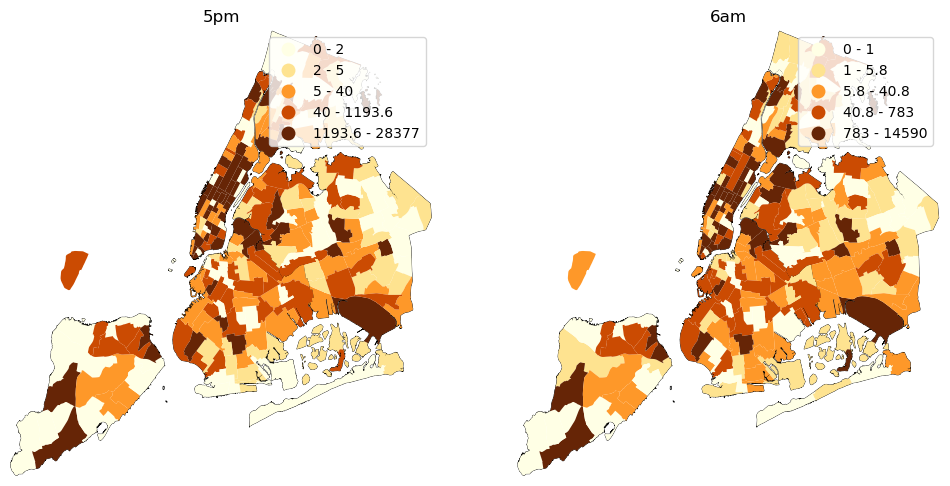
\includegraphics[width=0.95\textwidth]{plots/yellow_5pm_6am.png}
\centering
\caption{Yellow taxi pick-up times for each location in March 1 2016 in NYC}
\label{Fig:demand_loc_6am}
\end{subfigure}
\end{minipage}
\begin{minipage}{0.85\linewidth}
\begin{subfigure}{\linewidth}
\centering
\includegraphics[width=0.95\textwidth]{plots/green_5pm_6am.png}
\centering
\caption{Green taxi pick-up times for each location in March 1 2016 in NYC}
\label{Fig:demand_loc_6am}
\end{subfigure}
\end{minipage}
\end{figure}



In this report, we will analyse the taxi demand for pick-ups and drop-offs over spatial and temporal, simultaneously. A classic neural network model named LSTM \cite{sak2014long} is used in capturing the taxi demand structure over spatial and temporal in NYC and then used to predict the highest taxi demand location in real time.

The report is organised as follows. We first give a brief description of the datasets we use in section 2. Then we propose the analysis of taxi demand in one day by capturing the taxi demand structure over time and space.



% In this report, both yellow taxi and green taxi are used to analysis the taxi demand in NYC. Datasets are collected from 2016. 


\section{Dataset}
Datasets are collected from NYC Taxi \& Limousine Commission \footnote{\url{https://www1.nyc.gov/site/tlc/about/data-and-research.page}} which proposes the statistics about each taxi trip including pick-up location, drop-off location and so on. Both yellow and green taxis are used in this report to extract the taxi demand structure in one day over space and time. From January to December, we collected data on yellow taxis and green taxis. Finally, 131,131,805 trips are collected for yellow taxis and 16,385,541 for green taxis, respectively. Each trip is recorded by multiple features such as time, location, and trip distance, which provide sufficient information for us to learn about each trip well.

\subsection{Pre-processing}
We used datasets that recorded all taxi trips over yellow and green taxis with multiple features. To capture the structure of taxi demand across spatial and temporal scales, we must first identify the most representative features that have a significant impact on learning taxi demand structures in NYC. Thus, we first proposed the feature we used in section \ref{sec:feature_selection} and then we proposed the model we used in section \ref{sec:model}.

\subsubsection{Data filtering and time segmentation}
Remind that the aim of this report is to find the most correlated locations in different time. Thus, some noise data should be removed from the dataset which gains the consumption of modelling. 

We calculated the frequency of pick-up locations for yellow taxis in January 2016 at 5 pm. Figure \ref{Fig:time_loc_fre} shows the times of pick-up of yellow taxis in each location at 5pm in January 2016. As Figure \ref{Fig:time_loc_fre} shows, almost 75\% locations have little time of taxi demand, which can be considered as incidental trips. As a result, locations with less than 5 times pick-up are considered noise and are removed.By this way, the calculation of the model can be reduced and the bias be controlled.

As we can see in Figure \ref{Fig:demand_num}, the taxi demand is different at different times. Thus, we divided one day into four time segments, as shown in Table \ref{tab:time_seg}. In this way, the taxi demand has been further investigated since it shows a regular repetition.



\begin{figure}[ht]
\includegraphics[width=0.95\textwidth]{plots/time_loc_fre.pdf}
\centering
\caption{The number of pick-up demand for each location of yellow taxi in NYC at 5pm Jan 2016}
\label{Fig:time_loc_fre}
\end{figure}


\begin{table}[h]
\centering
\begin{tabular}{ll}
\hline
Time & Description \\\hline
6am to 9am &morning peak\\
9am to 5pm & daytime \\
5pm to 7pm & evening peak \\
7pm to 6am & nighttime \\\hline
\end{tabular}
\caption{Time segmentation in one day}
\label{tab:time_seg}
\end{table}



\subsubsection{Feature selection}
\label{sec:feature_selection}
Remind that the aim of this report is to find the most busy route between different areas in NYC to alleviate the transportation pressure. Thus, the features we care most about are spatial and temporal. Therefore, we focus on features that have the highest correlation with time and location.

The features we used are shown in Table \ref{tab:yellow_features} and Table \ref{tab:green_features} for yellow taxi and green taxi, respectively. For two reasons, we are more concerned about the pick-up time than the drop-off time. First, the pick-up time directly shows the taxi demand in a particular location during a particular time period. Second, drop-off time is more related to the traffic of the route network. Since then, we aim to learn which route is the most busy route in a certain time period. The pick-up time is when we care about it.



\begin{table}[h]
\centering
\begin{tabular}{ll}
\hline
Features & Description \\\hline
tpep\_pickup\_datetime&The date and time when the meter was engaged. \\
PULocationID & TLC Taxi Zone in which the taximeter was engaged.\\
DOLocationID&TLC Taxi Zone in which the taximeter was disengaged.\\\hline
\end{tabular}
\caption{Features used for yellow taxi.}
\label{tab:yellow_features}
\end{table}

 
\begin{table}[h]
\centering
\begin{tabular}{ll}
\hline
Features & Description \\\hline
lpep\_pickup\_datetime&The date and time when the meter was engaged. \\
PULocationID & TLC Taxi Zone in which the taximeter was engaged.\\
DOLocationID&TLC Taxi Zone in which the taximeter was disengaged.\\\hline
\end{tabular}
\caption{Features used for green taxi.}
\label{tab:green_features}
\end{table}

Features we use, such as ``lpep\_pickup\_datetime`` is collected with natural time, which cannot be directly used in the model. Thus, we do preparation for each feature. We consider one day as a basic time slot. For one day, one hour is a time slot, and time is labelled by natural time.
Then a trip can be represented as a tuple of time, pickup location, and drop-off location.

Given a time $t$, a pick-up location $l_{pick-up}$ and a drop-off location $l_{drop-off}$, we can obtain a tuple $\{$ $t$, $l_{pick-up}$, $l_{drop-off}$ $\}$. For trips in time $t$, we can establish a matrix $M_t$ where the row is pick-up location and the column is the drop-off location. The values in matrix $M_t$ is the times of the tuple $\{$ $t$, $l_{pick-up}$, $l_{drop-off}$ $\}$ appears. By constructing matrix for each hour, we can obtain a series of matrix which indicate the correlation between locations of taxi demand over time. Figure \ref{Fig:matrix} shows the construction of the matrix $M(t)$ in time $t$.

\begin{figure}[ht]
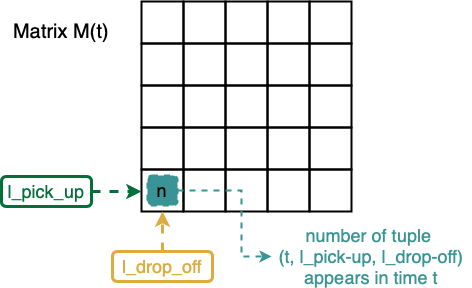
\includegraphics[width=0.55\textwidth]{plots/matrix.png}
\centering
\caption{The structure of matrix}
\label{Fig:matrix}
\end{figure}


\subsection{Model}
\label{sec:model}
We use one of the classic neural network models, long short-term memory recurrent neural network (LSTM) as our training model to find the most correlated locations in NYC for taxi demand over time \cite{sak2014long}. LSTM well reflects the sequential connections of data, which provides a promising option to model the correlation between locations during a time period.

The structure of the LSTM we used is shown in Figure \ref{Fig:LSTM}. The input of LSTM is the constructed matrix by time, pick-up location, and drop-off location. The output of LSTM is the probability of a top-correlated location between one location and other locations.



The coverage network is calculated by the following equation:
\begin{equation} \label{equ:C(s)}
C(T) =\sigma(W_s + b_s)
\end{equation}

The coverage network is then used to estimate the probability $P(T)$ of a location to be selected as the most related location in taxi service. Given $C(T)$, the probability score $P(T)$ is calculated by:
\begin{equation}
P(s) = softmax(W_sC_s + B_s)
\end{equation}
$B_s$ and $W_s$ are model parameters. 

\begin{figure}[ht]
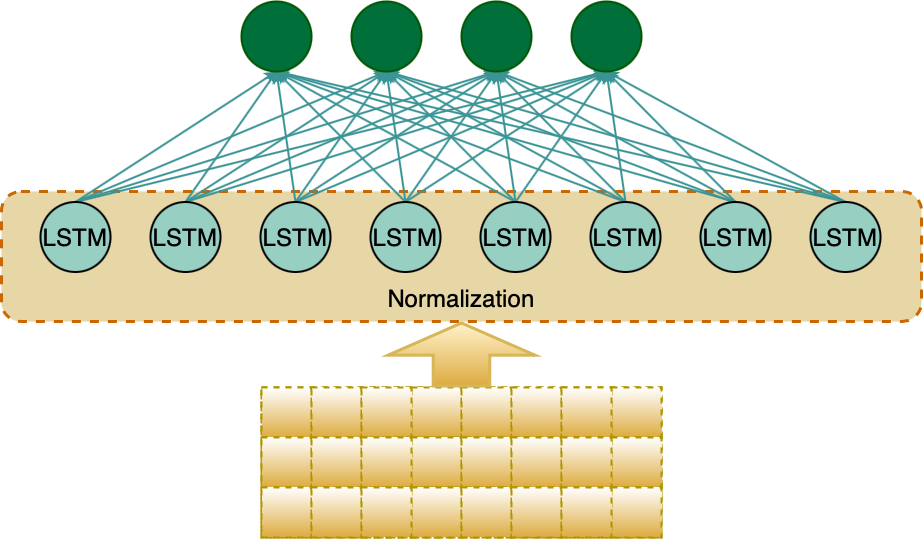
\includegraphics[width=0.75\textwidth]{plots/LSTM.png}
\centering
\caption{The structure of LSTM}
\label{Fig:LSTM}
\end{figure}


\section{Modelling}
In this section, we give the processing of modelling in the report. We first give the settings in modelling in section \ref{sec:setting}. Then we give the evaluation result in terms of time and workday in section \ref{sec:eff_time}.





\begin{figure}[h]
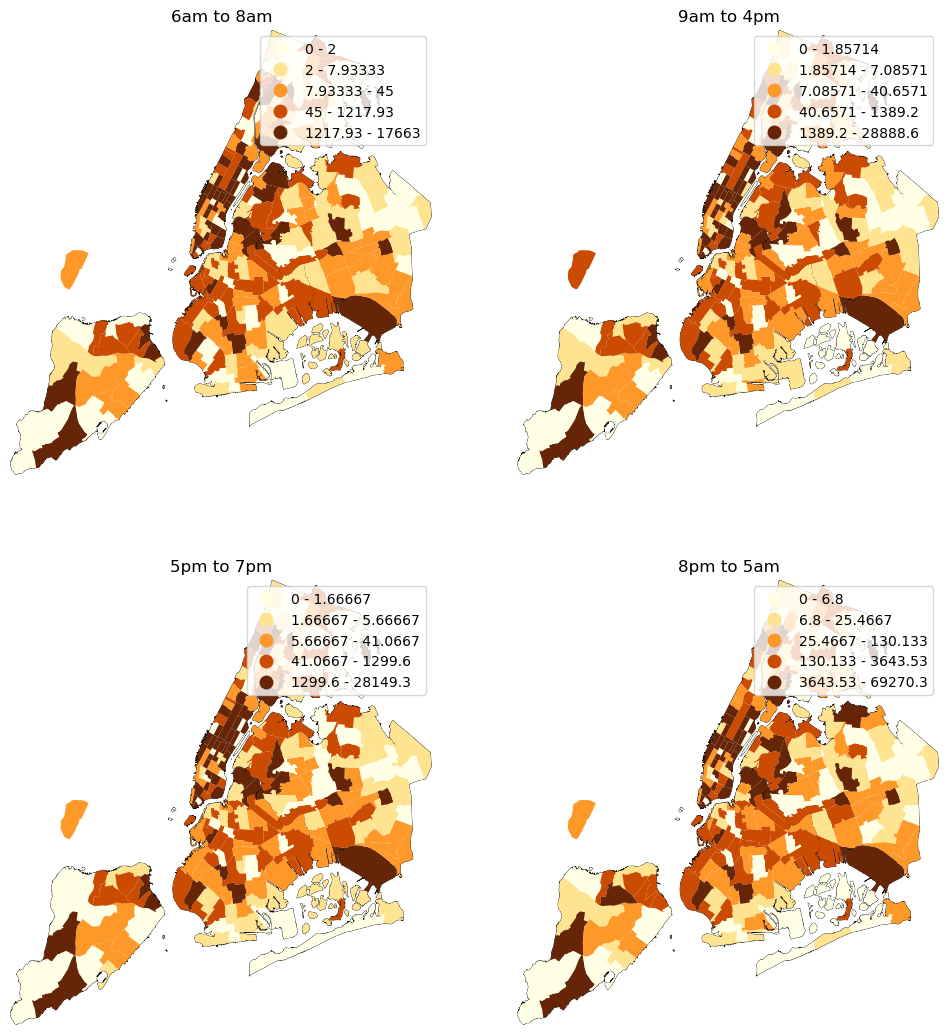
\includegraphics[width=0.75\textwidth]{plots/yellow_time_seg.png}
\centering
\caption{Yellow taxi demand in different time segmentation}
\label{Fig:yel_time}
\end{figure}

\subsection{Setting}
\label{sec:setting}
We use the proposed LSTM model in Figure \ref{Fig:LSTM} to find the pairwise locations which have the most correlation in trips. We employ the parameter settings in \cite{kim2020stepwise}. \cite{kim2020stepwise} aims to predict taxi demand in different area in a city using LSTM over yellow taxi. Thus, the number of LSTM units is set at 12. The batch size is set as 10. The number of iteration times is up to 500. We use Adam optimization and set the learning rate as 0.001.


\subsection{Effect of time segmentation}
\label{sec:eff_time}
We first used LSTM to find the most correlated locations in four time segments. Trips are divided according to time, as we proposed in section \ref{sec:feature_selection}.

Figure \ref{Fig:yel_time} and Figure \ref{Fig:green_time} show the average taxi demand per hour in NYC in these four time segments over yellow taxi and green taxi. As we can see, pickup locations with higher frequency are quite similar over both the morning peak and evening peak. This is because the population density somehow influences the taxi demand at different times. Moreover, within one hour, the higher taxi demand is always at the same locations. This is because taxi demand is highly related to population density in NYC.


\begin{figure}[ht]
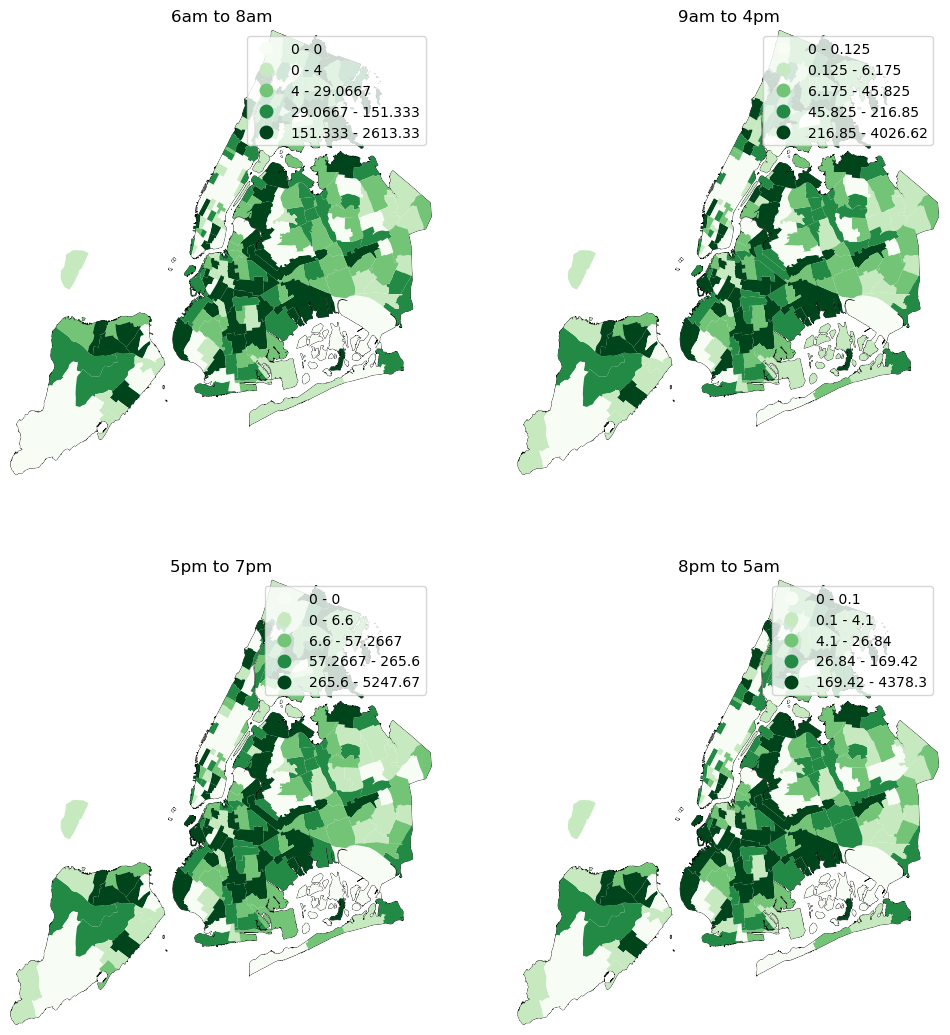
\includegraphics[width=0.75\textwidth]{plots/green_time_seg.png}
\centering
\caption{Green taxi demand in different time segmentation}
\label{Fig:green_time}
\end{figure}


\section{Conclusion}
In this report, we aim to find the most correlated locations for yellow and green taxis by capturing the most related trips between different taxi zones. We first collected data from TCL of yellow taxi and green taxi data in 2016, and then we selected features which are highly related to the task. Finally, three features are selected, time, pick-up location, and drop-off location. Time is divided into four segments to indicate the time impact of taxi demand. And finally, we use a classic neural network LSTM to find the most correlated locations in taxi trips.

This report shows that different locations have different taxi demand as shown in Figure \ref{Fig:demand_loc_6am} as well as time. By this observation, we suggest taxi drivers seek potential passengers in a certain location at a certain time. Furthermore, for a better transportation route network, more public transportation can be built between highly correlated locations. By this way, traffic in NYC could be improved by constructing proper public transportation.

The taxi demand also shows a difference in time segments. Both green and yellow cabs show a high demand in the daytime, especially in the morning peak and evening peak. Nighttime demand is much lower than it is in the daytime. Furthermore, green taxi demand is higher than yellow taxi demand in the suburbs, whereas yellow taxi demand shows the opposite in urban areas. This is because green taxis are more common on long trips.

In addition, we find that taxi demand is highly related to resident density. Comparing with population density in NYC \footnote{\url{http://www.undertheraedar.com/2012/01/population-density-in-new-york-city.html}}, the taxi demand is highly correlated to population density. Thus, for public service, population is the crucial factor of designing public transportation and decision making related to taxi demand.

\begin{figure}[h]
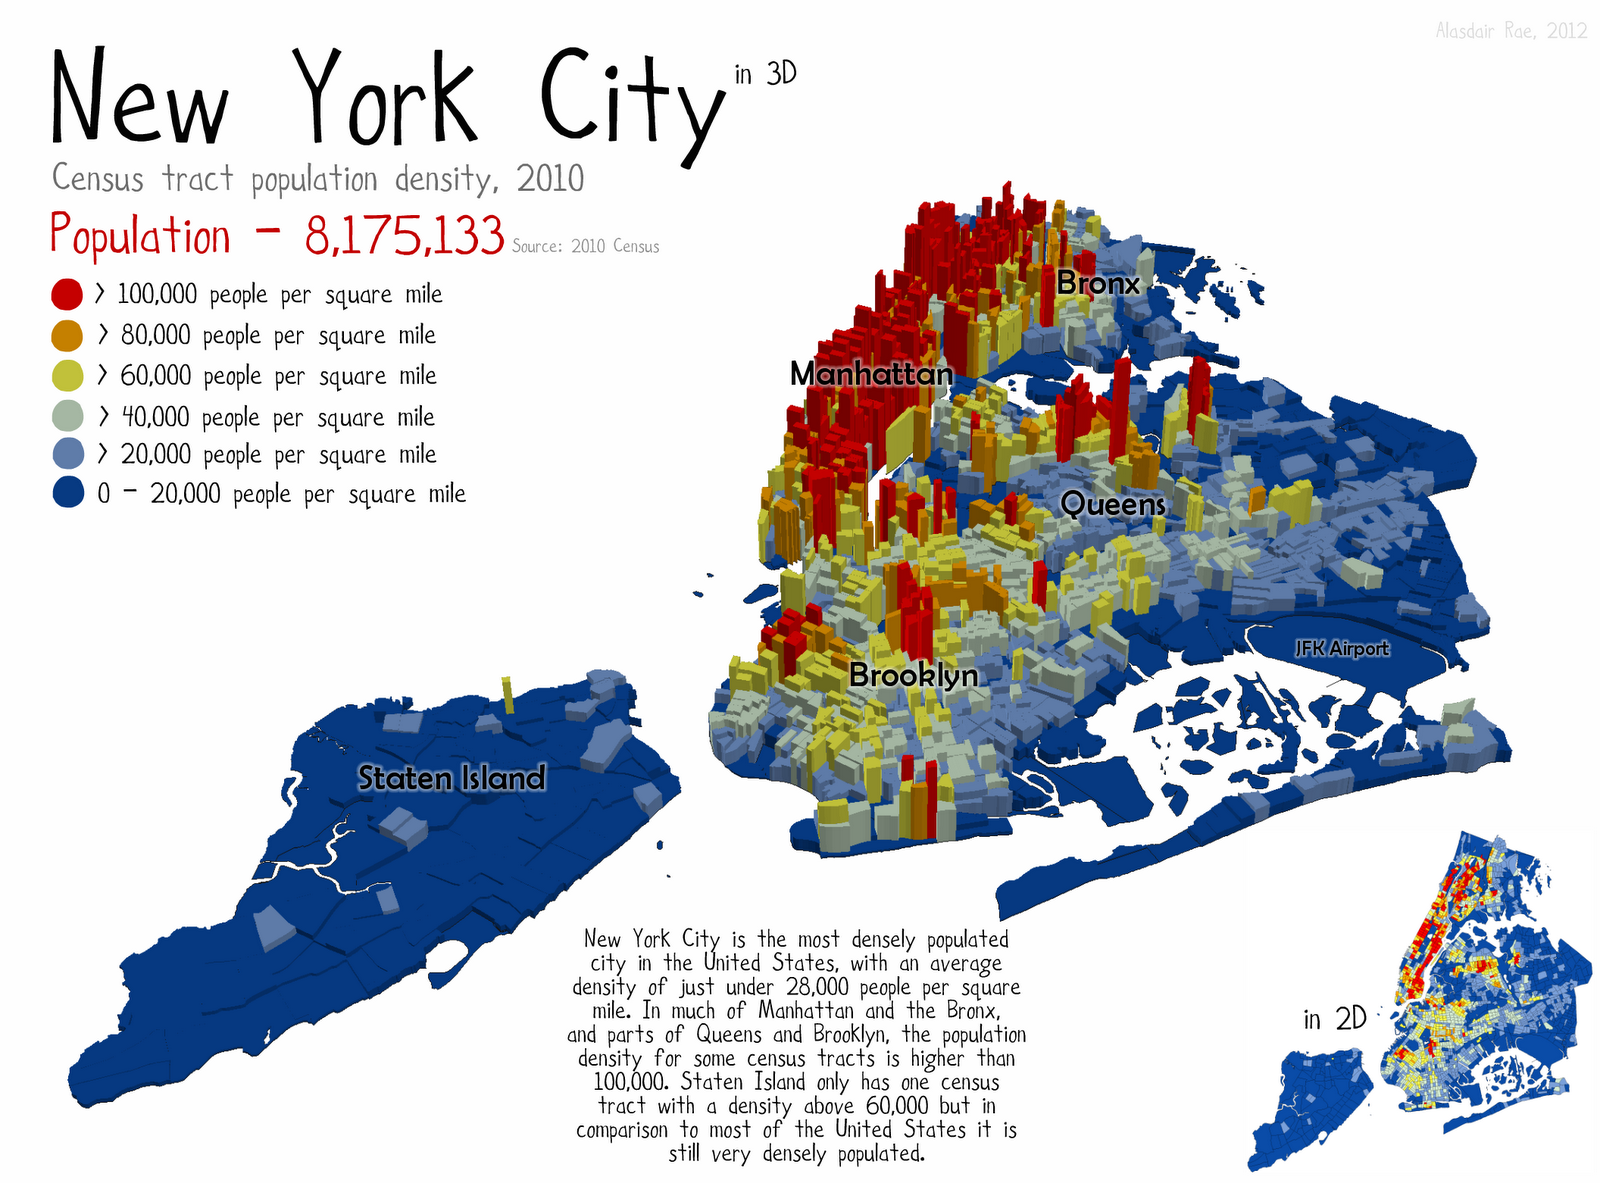
\includegraphics[width=0.65\textwidth]{plots/nyc_popdens_labels_layout2.png}
\centering
\caption{NYC population density in 2010 \footnote{\url{http://www.undertheraedar.com/2012/01/population-density-in-new-york-city.html}}}
\label{Fig:yel_time}
\end{figure}



\clearpage

% BEGIN REFERENCES SECTION
\printbibliography

\end{document}